\documentclass[12pt,utf8,notheorems,compress,t]{beamer}
\usepackage{etex}

\usepackage{pgfpages}
\setbeameroption{show notes on second screen}
\setbeamertemplate{note page}[plain]
\newcommand{\jnote}[2]{\only<#1>{\note{\setlength\parskip{\medskipamount}\justifying\footnotesize#2\par}}}

% Workaround for the issue described at
% https://tex.stackexchange.com/questions/164406/beamer-using-href-in-notes.
\newcommand{\fixedhref}[2]{\makebox[0pt][l]{\hspace*{\paperwidth}\href{#1}{#2}}\href{#1}{#2}}

\usepackage[english]{babel}

\usepackage{mathtools}
\usepackage{booktabs}
\usepackage{stmaryrd}
\usepackage{array}
\usepackage{ragged2e}
\usepackage{multicol}
\usepackage{tabto}
\usepackage{xstring}
\usepackage{ifthen}
\usepackage{soul}\setul{0.3ex}{}
\usepackage[all]{xy}
\xyoption{rotate}
\usepackage{tikz}
\usetikzlibrary{calc,shapes,shapes.callouts,shapes.arrows,patterns,fit,backgrounds,decorations.pathmorphing}
\hypersetup{colorlinks=true}

\usepackage{pifont}
\newcommand{\cmark}{\ding{51}}
\newcommand{\xmark}{\ding{55}}
\DeclareSymbolFont{extraup}{U}{zavm}{m}{n}
\DeclareMathSymbol{\varheart}{\mathalpha}{extraup}{86}

\graphicspath{{images/}}

\usepackage[protrusion=true,expansion=true]{microtype}

\setlength\parskip{\medskipamount}
\setlength\parindent{0pt}

\title{New reduction techniques in commutative algebra driven by logical methods}
\author{Ingo Blechschmidt}
\date{October 24th, 2018}

\useinnertheme[shadow=true]{rounded}
\setbeamerfont{block title}{size={}}

\useinnertheme{rectangles}

\usecolortheme{orchid}
\usecolortheme{seahorse}
\definecolor{mypurple}{RGB}{150,0,255}
\setbeamercolor{structure}{fg=mypurple}
\definecolor{myred}{RGB}{150,0,0}
\setbeamercolor*{title}{bg=myred,fg=white}
\setbeamercolor*{titlelike}{bg=myred,fg=white}
\setbeamercolor{frame}{bg=black}

\usefonttheme{serif}
\usepackage[T1]{fontenc}
\usepackage{libertine}

\newcommand{\A}{\mathcal{A}}
\newcommand{\B}{\mathcal{B}}
\newcommand{\M}{\mathcal{M}}
\renewcommand{\AA}{\mathbb{A}}
\newcommand{\E}{\mathcal{E}}
\newcommand{\F}{\mathcal{F}}
\renewcommand{\G}{\mathcal{G}}
\newcommand{\J}{\mathcal{J}}
\newcommand{\GG}{\mathbb{G}}
\renewcommand{\O}{\mathcal{O}}
\newcommand{\K}{\mathcal{K}}
\newcommand{\NN}{\mathbb{N}}
\newcommand{\QQ}{\mathbb{Q}}
\newcommand{\RR}{\mathbb{R}}
\newcommand{\TT}{\mathbb{T}}
\newcommand{\PP}{\mathbb{P}}
\newcommand{\ZZ}{\mathbb{Z}}
\newcommand{\CC}{\mathbb{C}}
\renewcommand{\P}{\mathcal{P}}
\newcommand{\aaa}{\mathfrak{a}}
\newcommand{\ppp}{\mathfrak{p}}
\newcommand{\fff}{\mathfrak{f}}
\newcommand{\defeq}{\vcentcolon=}
\newcommand{\defeqv}{\vcentcolon\equiv}
\newcommand{\Sh}{\mathrm{Sh}}
\newcommand{\GL}{\mathrm{GL}}
\newcommand{\Zar}{\mathrm{Zar}}
\newcommand{\op}{\mathrm{op}}
\newcommand{\Set}{\mathrm{Set}}
\newcommand{\Eff}{\mathrm{Ef{}f}}
\newcommand{\Sch}{\mathrm{Sch}}
\newcommand{\Aff}{\mathrm{Aff}}
\newcommand{\Ring}{\mathrm{Ring}}
\newcommand{\LocRing}{\mathrm{LocRing}}
\newcommand{\LRS}{\mathrm{LRS}}
\newcommand{\Hom}{\mathrm{Hom}}
\newcommand{\Spec}{\mathrm{Spec}}
\newcommand{\lra}{\longrightarrow}
\newcommand{\RelSpec}{\operatorname{Spec}}
\renewcommand{\_}{\mathpunct{.}}
\newcommand{\?}{\,{:}\,}
\newcommand{\speak}[1]{\ulcorner\text{\textnormal{#1}}\urcorner}
\newcommand{\ull}[1]{\underline{#1}}
\newcommand{\affl}{\ensuremath{{\ull{\AA}^1}}}
\newcommand{\Ll}{\vcentcolon\!\Longleftrightarrow}
\newcommand{\inv}{inv.\@}
\newcommand{\seq}{\vdash_{\!\!\!\vec x}}
\newcommand{\hg}{\mathbin{:}}  % homogeneous coordinates

\setbeamertemplate{blocks}[rounded][shadow=false]

\newenvironment{indentblock}{%
  \list{}{\leftmargin\leftmargin}%
  \item\relax
}{%
  \endlist
}

% Adapted from https://latex.org/forum/viewtopic.php?t=2251 (Stefan Kottwitz)
\newenvironment<>{hilblock}{
  \begin{center}
    \begin{minipage}{9.05cm}
      \setlength{\textwidth}{9.05cm}
      \begin{actionenv}#1
        \def\insertblocktitle{}
        \par
        \usebeamertemplate{block begin}}{
        \par
        \usebeamertemplate{block end}
      \end{actionenv}
    \end{minipage}
  \end{center}}

\newcommand{\bignumber}[1]{
  \renewcommand{\insertenumlabel}{#1}\scalebox{1.5}{\usebeamertemplate{enumerate item}}
}
\newcommand{\bigheart}{
\includegraphics{heart}}

\newenvironment{changemargin}[2]{%
  \begin{list}{}{%
    \setlength{\topsep}{0pt}%
    \setlength{\leftmargin}{#1}%
    \setlength{\rightmargin}{#2}%
    \setlength{\listparindent}{\parindent}%
    \setlength{\itemindent}{\parindent}%
    \setlength{\parsep}{\parskip}%
  }%
  \item[]}{\end{list}}

\tikzset{
  invisible/.style={opacity=0,text opacity=0},
  visible on/.style={alt={#1{}{invisible}}},
  alt/.code args={<#1>#2#3}{%
    \alt<#1>{\pgfkeysalso{#2}}{\pgfkeysalso{#3}}}
}

\newcommand{\pointthis}[3]{%
  \tikz[remember picture,baseline]{
    \node[anchor=base,inner sep=0,outer sep=0] (#2) {#2};
    \node[visible on=#1,overlay,rectangle callout,rounded corners,callout relative pointer={(0.3cm,0.5cm)},fill=blue!20] at ($(#2.north)+(-0.1cm,-1.1cm)$) {#3};
  }%
}

% Adapted from https://latex.org/forum/viewtopic.php?t=2251 (Stefan Kottwitz)
\newenvironment<>{varblock}[2]{\begin{varblockextra}{#1}{#2}{}}{\end{varblockextra}}
\newenvironment<>{varblockextra}[3]{
  \begin{center}
    \begin{minipage}{#1}
      \begin{actionenv}#4
        {\centering \hil{#2}\par}
	\def\insertblocktitle{}%\centering #2}
        \def\varblockextraend{#3}
	\usebeamertemplate{block begin}}{
        \par
        \usebeamertemplate{block end}
        \varblockextraend
      \end{actionenv}
    \end{minipage}
  \end{center}}

\setbeamertemplate{frametitle}{%
  \vskip1.2em%
  \leavevmode%
  \begin{beamercolorbox}[dp=1ex,center]{}%
      \usebeamercolor[fg]{item}{\textbf{{\Large \insertframetitle}}}
  \end{beamercolorbox}%
}

\setbeamertemplate{navigation symbols}{}

\newcounter{framenumberpreappendix}
\newcommand{\backupstart}{
  \setcounter{framenumberpreappendix}{\value{framenumber}}
}
\newcommand{\backupend}{
  \addtocounter{framenumberpreappendix}{-\value{framenumber}}
  \addtocounter{framenumber}{\value{framenumberpreappendix}} 
}

\newcommand{\mynav}[3]{%
  \begin{beamercolorbox}[wd=\paperwidth,ht=2.25ex]{}%
    \begin{columns}
      \begin{column}{0.333\textwidth}
        \raggedright
        \textcolor{#1}{\qquad\qquad Summary}
        \par
      \end{column}
      \begin{column}{0.333\textwidth}
        \centering
        \textcolor{#2}{The forcing model}
        \par
      \end{column}
      \begin{column}{0.333\textwidth}
        \raggedleft
        \textcolor{#3}{Revisiting the test cases \qquad\qquad}
        \par
      \end{column}
    \end{columns}
  \end{beamercolorbox}%
}

\newcommand{\insertframeextra}{}
\setbeamertemplate{footline}{%
  \begin{beamercolorbox}[wd=\paperwidth,ht=2.25ex,dp=1ex,right,rightskip=1mm,leftskip=1mm]{}%
    % \inserttitle
    \hfill
    \insertframenumber\insertframeextra\,/\,\inserttotalframenumber
  \end{beamercolorbox}%
  \vskip0pt%
}


\newcommand{\hil}[1]{{\usebeamercolor[fg]{item}{\textbf{#1}}}}
\newcommand{\bad}[1]{\textcolor{red!90}{\textnormal{#1}}}

\begin{document}

\addtocounter{framenumber}{-1}

\setbeamertemplate{headline}{\mynav{gray}{gray}{gray}}

{\usebackgroundtemplate{\begin{minipage}{\paperwidth}\vspace*{4.95cm}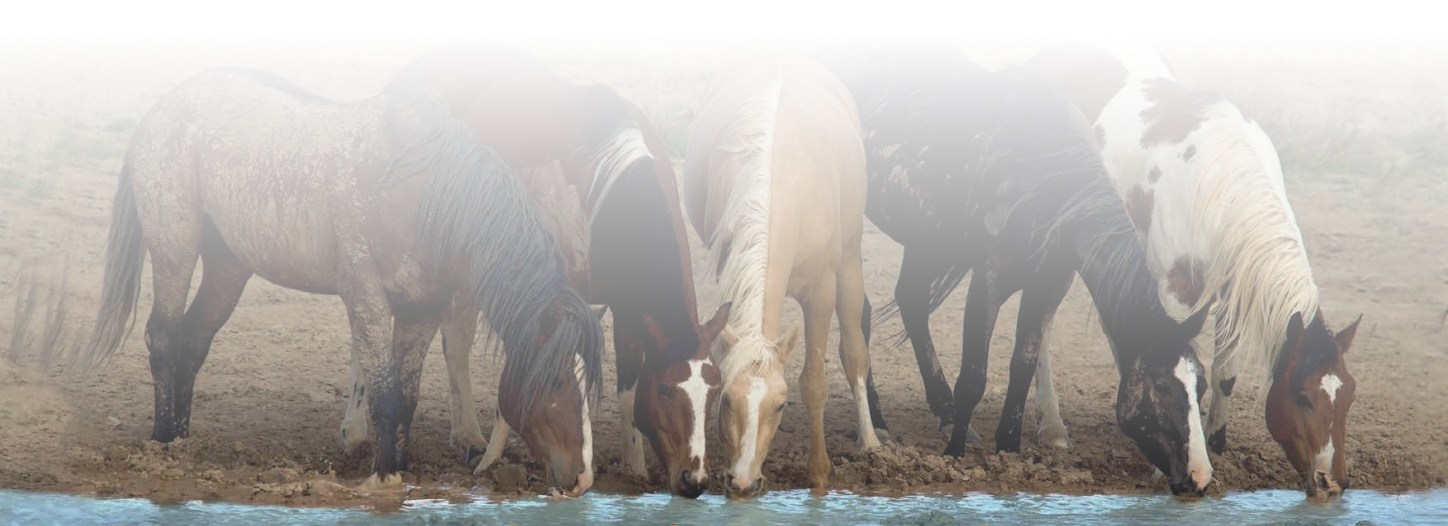
\includegraphics[width=\paperwidth]{topos-horses}\end{minipage}}
\begin{frame}[c]
  \centering

  \bigskip
  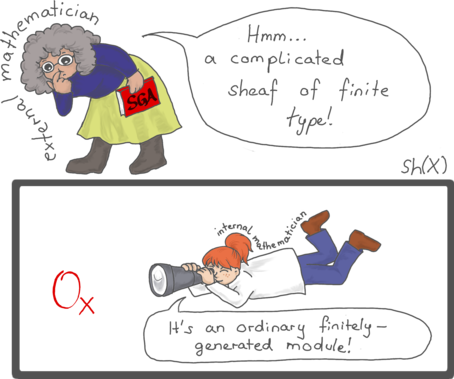
\includegraphics[width=0.4\textwidth]{external-internal-small}
  \bigskip

  \hil{New reduction techniques in commutative algebra driven by logical methods}

  \scriptsize
  \textit{-- an invitation --}
  \bigskip

  Ingo Blechschmidt \\
  Università di Verona
  \bigskip

  Logic Seminar Padova \\
  December 5st, 2018
  \par

  \jnote{1}{We can associate to any reduced ring~$A$ a \emph{forcing
  model}~$A^\sim$.
  \begin{itemize}
    \item The forcing model has the pleasant property that it is a field.
    \item Reasoning about it requires that we restrict ourselves to
    intuitionistic logic.
  \end{itemize}
  Details are on the following slides.}
\end{frame}}


\section{Summary}
\setbeamertemplate{headline}{\mynav{black}{gray}{gray}}

\begin{frame}{Summary}
  \vspace*{-1em}

  \visible<4->{
    \begin{changemargin}{-2.0em}{-0.5em}
      \begin{itemize}
        \item \ \\[-1.2em]\mbox{For any reduced ring~$A$, there is a ring~$A^\sim$ in a certain topos with}
        \[ \models \bigl(\forall x\?A^\sim\_ \neg(\exists y\?A^\sim\_ xy = 1) \Rightarrow x = 0\bigr). \]

        \item This semantics is sound with respect to intuitionistic logic.

        \item \ \\[-1.2em]\mbox{It has uses in classical and constructive commutative
        algebra.}
      \end{itemize}
    \end{changemargin}
  }

  \vspace*{-1.5em}

  \begin{columns}[t]
    \begin{column}[t]{0.52\textwidth}
      \centering

      \begin{varblock}{\textwidth}{A baby example}
        \justifying
        Let~$M$ be an injective matrix with more columns than rows over a
        reduced ring~$A$.
        Then~$1 = 0$ in~$A$.
      \end{varblock}
      \vspace*{-0.5em}

      \only<1>{
        \scalebox{0.8}{$\begin{pmatrix}
          \cdot & \cdot & \cdot & \cdot & \cdot \\
          \cdot & \cdot & \cdot & \cdot & \cdot \\
          \cdot & \cdot & \cdot & \cdot & \cdot
        \end{pmatrix}$}
      }

      \visible<2->{
        \justifying
        \textbf{Proof.} \bad{Assume not.} Then there is a \bad{minimal
        prime ideal} $\ppp \subseteq A$. The matrix is injective over the \bad{field}~$A_\ppp = A[(A
        \setminus \ppp)^{-1}]$; contradiction to basic linear algebra.
      }
    \end{column}

    \begin{column}[t]{0.46\textwidth}
      \centering

      \begin{varblock}{\textwidth}{Generic freeness\phantom{p}}
        \justifying
        Generically, any finitely generated module over a reduced ring
        is free.\phantom{g}
      \end{varblock}
      \vspace*{-0.5em}

      \only<1-2>{{
        \scriptsize\raggedright
        (A ring is reduced iff $x^n=0$ implies $x=0$.)
        \par
      }}

      \only<1-2>{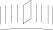
\includegraphics[width=0.73\textwidth]{generic-freeness}}

      \visible<3->{
        \justifying
        \textbf{Proof.} See \href{https://stacks.math.columbia.edu/tag/051Q}{[Stacks Project]}.
      }
    \end{column}
  \end{columns}

  \jnote{1}{The two displayed statements are trivial for fields. It is
  therefore natural to try to reduce the general situation to that of fields.}

  \jnote{2}{The displayed proof, which could have been taken from any
  standard textbook on commutative algebra, succeeds in this reduction
  by employing proof by contradiction and minimal prime ideals. However, this way
  of reducing comes at a cost: It requires the Boolean Prime Ideal Theorem
  (for ensuring the existence of a prime ideal and for ensuring that stalks at
  minimal prime ideals are fields) and even the full axiom of choice (for
  ensuring the existence of a minimal prime ideal).

  We should hope that such a simple statement admits a more informative,
  explicit, computational proof not employing transfinite methods: There should
  be an explicit method for
  transforming the given conditional equations expressing injectivity into the
  equation~$1 = 0$. And indeed there is: Beautiful constructive proofs can
  be found in Richman's note on
  \fixedhref{https://www.ams.org/journals/proc/1988-103-04/S0002-9939-1988-0954974-5/S0002-9939-1988-0954974-5.pdf}{nontrivial
  uses of trivial rings} and in the
  \fixedhref{https://arxiv.org/abs/1605.04832}{recent textbook by Lombardi and
  Quitté} on constructive commutative algebra.

  The new reduction technique presented in this talk provides a way of
  performing the reduction in an entirely constructive manner, avoiding the
  axiom of choice. If so desired, resulting topos-theoretic proofs can be
  unwound to yield fully explicit, topos-free, direct proofs.}

  \jnote{3}{The baby example demonstrates that the reduction technique of this
  talk is of interest to constructive commutative algebra. What about classical
  commutative algebra? This is what the second example aims at.
  Grothendieck's generic freeness lemma is an important theorem in algebraic
  geometry, where it is usually stated in the following geometric form:

  \vspace*{-1.2em}
  \begin{indentblock}Let~$X$ be a reduced scheme. Let~$\B$ be
  an~$\O_X$-algebra of finite type. Let~$\M$ be a~$\B$-module of finite type.
  Then over a dense open,
  \begin{enumerate}
  \item[(a)] $\B$ and~$\M$ are locally free as sheaves of~$\O_X$-modules,
  \item[(b)] $\B$ is of finite presentation as a sheaf of~$\O_X$-algebras and
  \item[(c)] $\M$ is of finite presentation as a sheaf of~$\B$-modules.
  \end{enumerate}\end{indentblock}
  \vspace*{-1.2em}

  All previously known proofs proceed in a series of reduction steps,
  finally culminating in the case where~$A$ is a Noetherian integral domain.
  They are somewhat convoluted (spanning several pages) and require nontrivial
  prerequisites in commutative algebra.

  Using the new reduction technique, there is a short (one-paragraph) and
  conceptual proof of Grothendieck's generic freeness lemma. It is constructive
  as a bonus; and if desired, one can unwind the resulting proof to obtain a
  constructive proof which doesn't reference topos theory. The proof obtained
  in this way is still an improvement on the previously known proofs, requiring
  no advanced prerequisites in commutative algebra, and takes
  \fixedhref{https://arxiv.org/abs/1807.01231}{about a page}.}

  \jnote{4}{Instead of passing from a given ring~$A$ to one of its
  stalks~$A_\ppp$ or quotient rings~$A/\aaa$, the reduction technique presented
  in this talk passes from~$A$ to a \emph{forcing model}~$A^\sim$.

  Unlike stalks or quotient rings, which are honest rings, the forcing
  model~$A^\sim$ is not a ring in the strict sense of the word: It doesn't
  have an underlying \emph{set} of elements, but instead an underlying
  \emph{sheaf} of elements. It is a \emph{ring object} in a certain category,
  the \emph{little Zariski topos} of~$A$. But as long as we restrict to intuitionistic
  reasoning, this difference is immaterial. A metatheorem displayed on a later
  slide states that any intuitionistic theorem about
  rings applies to~$A^\sim$ just as if~$A$ were a proper, ordinary ring.
  
  Studying~$A^\sim$ is in fact the same as studying~$A$ from a certain
  different, \emph{local} point of view. The precise meaning of this statement
  will be explained on slide~3.}

  \jnote{5}{Intuitionistic logic is the same as classical logic, but without:
  \vspace*{-1em}
  \begin{itemize}
    \item the law of excluded middle: $\varphi \vee \neg\varphi$ \\[-1.5em]
    \item the law of double negation elimination: $\neg\neg\varphi \Rightarrow \varphi$ \\[-1.5em]
    \item the axiom of choice
  \end{itemize}
  \vspace*{-1em}
  If one is unfamiliar with constructive mathematics, then doing without these
  three laws seems unmotivated, rather peculiar and overtly restrictive. Here, the
  restriction to intuitionistic logic is not by some philosophical choice.
  Rather, it's by mathematical necessity. It's just a fact that in general, the
  laws of classical logic don't apply to~$A^\sim$. (Assuming a classical
  metatheory and assuming~$A$ to be Noetherian, they do iff~$A$ is of Krull
  dimension~$\leq 0$.)

  Luckily, vast amounts of commutative algebra work in the intuitionistic
  setting, as for instance evidenced by the recent 1000$^+$-page
  \fixedhref{https://arxiv.org/abs/1605.04832}{textbook by
  Lombardi and Quitté}. This claim extends to statements which are usually
  proven using maximal ideals or minimal ideal prime ideals and hence require
  Zorn's lemma. Indeed, the technique presented in this talk allows to
  constructivize some results of this kind.
 
  Background on constructive mathematics can for instance be found in a
  \fixedhref{https://video.ias.edu/members/1213/0318-AndrejBauer}{talk by
  Andrej Bauer}
  (\fixedhref{https://www.ams.org/journals/bull/2017-54-03/S0273-0979-2016-01556-4/S0273-0979-2016-01556-4.pdf}{written
  notes}). The standard proof that~$\sqrt{2}$ is not rational is perfectly fine
  in constructive mathematics.}
\end{frame}


\section{The forcing model}
\setbeamertemplate{headline}{\mynav{gray}{black}{gray}}

\begin{frame}{Motivating the semantics}
  \centering
  \begin{varblockextra}{0.8\textwidth}{}{
    \hil{Examples:}\phantom{Non-}\,\!\ \ $k,\ k[[X]],\ \CC\{z\},\ \ZZ_{(p)}$ \\[0.2em]
    \hil{Non-examples:}\ \ $\ZZ,\ k[X],\ \ZZ/(pq)$
  }
    \justifying
    A ring is \hil{local} iff~$1 \neq 0$ and if~$x + y = 1$ implies that~$x$ is
    invertible or~$y$ is invertible.
  \end{varblockextra}

  \begin{varblockextra}{0.8\textwidth}{}{
    Let~$x + y = 1$ in a ring~$A$.
    Then:
    \begin{itemize}
      \item The element $x$ is invertible in~$A[x^{-1}]$.
      \item The element $y$ is invertible in~$A[y^{-1}]$.
    \end{itemize}
    (Recall~$A[f^{-1}] = \bigl\{ \frac{u}{f^n} \,|\, u \in A, n \in \NN \bigr\}$.)
  }
    \hil{Locally,} any ring is local.
  \end{varblockextra}

  \jnote{1}{In topos theory, we have lots of experience of \emph{changing
  universes} in order to \emph{force} some statements to become true. However,
  because the field condition we are aiming at is not a \emph{geometric
  sequent}, these techniques do not work here. Hence we'll take it more slowly
  and only devise a semantics which forces the given ring to be local.

  The displayed definition of a local ring is, in the presence of the axiom of
  choice, equivalent to the more common one (ring with exactly one maximal
  ideal). In constructive mathematics, the displayed definition usually works
  better.

  The key insight is that \emph{locally} (in the sense of topology/geometry),
  any ring is a local ring. That is, we may pretend that any given ring is
  local if we are prepared to pass to numerous localizations during the course
  of an argument. The semantics displayed on the next slide manages this
  localization-juggling for us.

  By~$A[f^{-1}]$, we mean the localization of~$A$ away from~$f$. This
  construction makes sense even if~$f$ is a zero divisor, in which
  case~$A[f^{-1}]$ is the zero ring.}
\end{frame}

\begin{frame}{The Kripke--Joyal semantics}
  \small\vspace*{-0.7em}
  \only<1>{Let~$A$ be a ring (commutative, with unit). We recursively define
  \[ f \models \varphi \quad \text{(``$\varphi$ holds away from the zeros of~$f$'')} \]
  for elements~$f \in A$ and statements~$\varphi$. Write
  ``$\models \varphi$'' to mean~$1 \models \varphi$.}
  \only<1>{\[ \renewcommand{\arraystretch}{1.25}\begin{array}{@{}l@{\quad}c@{\quad}l@{}}
    f \models \top &\text{is}& \text{true} \\
    f \models \bot &\text{iff}& \text{$f$ is nilpotent} \\
    f \models x = y &\text{iff}& x = y \in A[f^{-1}] \\
    f \models \varphi \wedge \psi &\text{iff}&
      \text{$f \models \varphi$ and $f \models \psi$} \\
    f \models \varphi \vee \psi &\text{iff}&
      \text{there exists a partition~$f^n = fg_1 + \cdots + fg_m$ with,} \\
    &&\quad\text{for each~$i$, $fg_i \models \varphi$ or $fg_i \models \psi$} \\
    f \models \varphi \Rightarrow \psi &\text{iff}&
      \text{for all~$g \in A$, $fg \models \varphi$ implies $fg \models \psi$} \\
    f \models \forall x\?A^\sim\_ \varphi &\text{iff}&
      \text{for all~$g \in A$ and all $x_0 \in A[(fg)^{-1}]$, $fg \models \varphi[x_0/x]$} \\
    f \models \exists x\?A^\sim\_ \varphi &\text{iff}&
      \text{there exists a partition~$f^n = fg_1 + \cdots + fg_m$ with,} \\
    &&\quad\text{for each~$i$, $fg_i \models \varphi[x_0/x]$ for some~$x_0 \in A[(fg_i)^{-1}]$}
  \end{array} \]}
  \only<2->{Write ``$\models \varphi$'' to mean~$1 \models \varphi$.}
  \only<2->{\[ \renewcommand{\arraystretch}{1.25}\begin{array}{@{}l@{\quad}c@{\quad}l@{}}
    f \models x = y &\text{iff}& x = y \in A[f^{-1}] \\
    f \models \varphi \wedge \psi &\text{iff}&
      \text{$f \models \varphi$ and $f \models \psi$} \\
    f \models \varphi \vee \psi &\text{iff}&
      \text{there exists a partition~$f^n = fg_1 + \cdots + fg_m$ with,} \\
    &&\quad\text{for each~$i$, $fg_i \models \varphi$ or $fg_i \models \psi$}
  \end{array} \]}

  \jnote{1}{The clause for~``$\vee$'' is made exactly in such a way as to
  ensure, if~$x + y = 1$, that~$1 \models ((\exists z\?A^\sim\_ xz = 1) \vee
  (\exists z\?A^\sim\_ yz = 1))$.
  
  The definition of the semantics is reminiscent of Kripke and Beth models.
  Indeed, it is a fragment of the Kripke--Joyal semantics of the \emph{internal
  language of a topos}, and this general semantics encompasses Kripke and Beth
  models as special cases.}

  \jnote{2}{The soundness lemma states: If~$f \models \varphi$, and
  if~$\varphi$ intuitionistically entails a further statement~$\psi$, then
  also~$f \models \psi$. In this way we can \emph{reason} with the forcing
  model, similarly as if~$A^\sim$ would actually exist as a ring instead of
  merely being a convenient syntactic fiction.

  If we want~$A^\sim$ to actually exist, not just as a figure of speech, then
  we have to broaden our notion of existence and accept ring objects in
  toposes. More on this on the next slide.

  The four lemmas displayed on this slide, as well as all the claims on
  further slides, can be proven in very weak intuitionistic metatheories.}

  \jnote{3}{Irrespective of whether~$A$ is a local ring, its mirror
  image~$A^\sim$ is always a local ring (that is, the axioms of what it means
  to be a local ring hold under the translation rules specified by the
  semantics). A basic application of this forcing model are local-to-global
  principles. For instance:
  \begin{itemize}\justifying
    \item The statement ``the kernel of a surjective matrix over a local ring
    is finite free'' admits a constructive proof. It therefore holds
    for~$A^\sim$. Its external meaning is that the kernel of a surjective
    matrix~$M$ over~$A$ is finite locally free (there exists a partition~$1 =
    f_1 + \cdots + f_n$ such that for each~$i$, the localized
    module~$(\operatorname{ker} M)[f_i^{-1}]$ is finite free).

    \item The ring~$A$ is a Prüfer domain if and only if~$A^\sim$ is a Bézout
    domain. Therefore any constructive theorem about Bézout domains entails a
    corresponding theorem about Prüfer domains. Bézout domains are quite rare,
    while Prüfer domains abound (for instance the ring of integers of any
    number field is a Prüfer domain, even constructively so).
  \end{itemize}}

  \pause

  \begin{columns}
    \begin{column}{0.50\textwidth}
      \begin{varblock}{\textwidth}{Monotonicity}{}
        If~$f \models \varphi$, then also~$fg \models \varphi$.
      \end{varblock}
    \end{column}

    \begin{column}{0.50\textwidth}
      \begin{varblock}{\textwidth}{Locality}{}
        \justifying
        If~$f^n = fg_1 + \cdots + fg_m$ and~$fg_i \models \varphi$ for all~$i$,
        then also~$f \models \varphi$.
      \end{varblock}
    \end{column}
  \end{columns}

  \begin{columns}
    \begin{column}{0.50\textwidth}
      \begin{varblock}{\textwidth}{Soundness\phantom{p}}{}
        If~$\varphi \vdash \psi$ and~$f \models \varphi$,
        then~$f \models \psi$.
      \end{varblock}
    \end{column}

    \begin{column}{0.50\textwidth}
      \begin{varblock}{\textwidth}{Forced properties}{}
        $\models \speak{$A^\sim$ is a local ring}$.
      \end{varblock}
    \end{column}
  \end{columns}
\end{frame}

\tikzstyle{topos} = [draw=mypurple, very thick, rectangle, rounded corners, inner sep=5pt, inner ysep=10pt]
\tikzstyle{title} = [fill=mypurple, text=white]

% Taken from Todd Lehman (CC-BY-SA) at https://tex.stackexchange.com/a/44920/32372

\newcommand{\setisprime}[1]{
  % Sets \isprime based on #1.
  \ifnum#1=1 \gdef\isprime{0} \else \gdef\isprime{1} \fi
  \foreach \sip in {2, 3,5,...,#1} {
    \pgfmathparse{\sip*\sip>#1? 1:0}
    \ifthenelse{\pgfmathresult=1}{
      % Early-out if \sip^2 > #1.
      \breakforeach
    }{
      % Otherwise test if \sip divides #1.
      \pgfmathparse{Mod(#1,\sip)==0? 1:0}
      \ifthenelse{\pgfmathresult=1}{
        \gdef\isprime{0}
        \breakforeach
      }{}
    }
  }
}

\newcommand{\setxy}[1]{
  % Sets \x and \y to loction of cell #1.
  \pgfmathtruncatemacro{\x}{Mod(#1-1,\cols)}
  \pgfmathtruncatemacro{\y}{(#1-1) / \cols}
  \pgfmathtruncatemacro{\y}{\cols - 1 - \y}
  \pgfmathparse{2.5*(\x+.5)}\let\x\pgfmathresult
  \pgfmathparse{2.5*(\y+.5)}\let\y\pgfmathresult
}

\newcommand{\numlabel}[2]{
  % Draws label #2 at cell #1.
  \setxy{\n}
  \node[fill=none, text=black] at (\x,\y) {#2};
}

\newcommand{\drawpolygon}[2]{
  % Draws polygon with #2 vertexes at cell #1.
  \setxy{#1}
  \ifthenelse{#2>1}{ % Polygon must have at least 2 sides.
    \ifthenelse{#2<30}{ % Draw polygon if it has a small number of sides.
      \filldraw (\x,\y) +(90:1)
      \foreach \drawi in {1,...,#2} {-- +(\drawi/#2*360+90:1)} -- cycle;
    }{ % Else approximate with circle.
      \filldraw (\x,\y) circle(1);
    }
  }{}
}

\newcommand{\setpolygoncolor}[1]{
  % Sets color based on #1.
  \gdef\polycolor{black}
  \ifnum#1=2\gdef\polycolor{black!50!white}\fi
  \ifnum#1=3\gdef\polycolor{yellow!95!red}\fi
  \ifnum#1=5\gdef\polycolor{yellow!0!red}\fi
  \ifnum#1=7\gdef\polycolor{blue!75!green}\fi
  \ifnum#1=11\gdef\polycolor{blue!70!red}\fi
  \ifnum#1=13\gdef\polycolor{blue!40!red}\fi
  \ifnum#1=17\gdef\polycolor{green!50!blue}\fi
  \ifnum#1=19\gdef\polycolor{green!80!black}\fi
  \ifnum#1=23\gdef\polycolor{green!50!red}\fi
  \ifnum#1=29\gdef\polycolor{yellow!50!black}\fi
  \ifnum#1=31\gdef\polycolor{orange!50!black}\fi
  \ifnum#1=37\gdef\polycolor{red!50!black}\fi
  \ifnum#1=41\gdef\polycolor{purple!50!black}\fi
  \ifnum#1=43\gdef\polycolor{blue!50!black}\fi
  \ifnum#1=47\gdef\polycolor{green!50!black}\fi
  \ifnum#1=53\gdef\polycolor{white!50!black}\fi
  \ifnum#1=59\gdef\polycolor{white!50!black}\fi
  \ifnum#1=61\gdef\polycolor{white!50!black}\fi
  \ifnum#1=67\gdef\polycolor{white!50!black}\fi
}

\newcommand{\sieve}[2]{
  \def\cols{#1}
  \def\rows{#2}
  \begin{tikzpicture}[scale=.5]
  \pgfmathtruncatemacro{\nmax}{\rows * \cols}

  \foreach \n in {1,...,\nmax} {
    \begin{scope}[fill=gray, fill opacity=.05,
                  draw=gray, draw opacity=.10,
                  line width=4]
      \drawpolygon{\n}{\n}
    \end{scope}
    \setisprime{\n}
    \ifthenelse{\isprime=1}{
      \numlabel{\n}{\bf\n}
    }{
      \def\startintensity{.33}
      \def\incrintensity{.10}
      \def\intensity{\startintensity}

      \def\m{\n}
      \pgfmathtruncatemacro{\i}{\m / 2}

      % Divide \m by \i until \m is extinguished.
      % Increment \i each time it does not divide into \m.
      \whiledo{\m>1}{
        \setisprime{\i}
        \pgfmathparse{Mod(\m,\i)==0? 1:0}
        \ifthenelse{\pgfmathresult=1\and\isprime=1}{
          \setpolygoncolor{\i}
          \begin{scope}[fill=\polycolor, fill opacity=\intensity,
                        draw=\polycolor!85!black, draw opacity=\intensity,
                        line width=\intensity*1.5]
            \drawpolygon{\n}{\i}
          \end{scope}
          \pgfmathtruncatemacro{\m}{\m / \i}
          \pgfmathparse{\intensity + \incrintensity}\let\intensity\pgfmathresult
        }{
          \pgfmathtruncatemacro{\i}{\i - 1}
          \def\intensity{\startintensity}
        }
      }
      \begin{scope}[text=black, text opacity=.5]
        \numlabel{\n}{\scriptsize\n}
      \end{scope}
    }
  }

  \end{tikzpicture}
}

%\renewcommand{\sieve}[2]{SIEVE}
%\renewcommand{\fakesieve}[2]{SIEVE}

\newcommand{\drawbox}[4]{
  \node[topos, #4] [fit = #3] (#1) {};
  \node[title] at (#1.north) {#2};
}

\newcommand{\muchstuff}{
  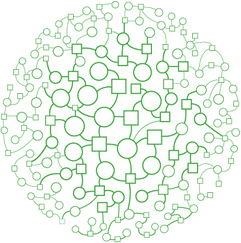
\includegraphics[height=3em]{filmat}
  \scalebox{0.5}{\sieve{14}{2}}
}

\newcommand{\muchstuffplaceholder}{
  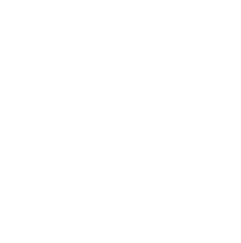
\includegraphics[height=3em]{filmat-placeholder}
  \scalebox{0.5}{\fakesieve{14}{2}}
}

\newcommand{\fewstuff}{
  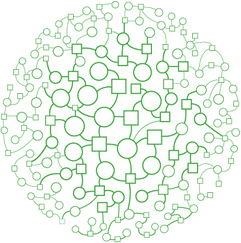
\includegraphics[height=3em]{filmat}
  \scalebox{0.5}{\sieve{7}{2}}
}

\begin{frame}[fragile]{A universal property}
  The displayed semantics is the first-order fragment of the \hil{higher-order
  internal language} of the \hil{little Zariski topos}.

  \begin{tikzpicture}
    \node[scale=0.4] (objs-set1) at (-4.0,-2.5) {
      \only<1->{\fewstuff}
    };
    \node[scale=0.4] (objs-eff1) at (4.0,-2.5) {
      \only<1->{\fewstuff}
    };
    \node[scale=0.4] (objs-sh1)  at (0,-2.5) {
      \only<1->{\fewstuff}
    };

    \node (prop-set1) [below of=objs-set1, align=left, inner ysep=0pt] {
      The usual laws \\
      of logic hold.
    };

    \node (prop-eff1) [below of=objs-eff1, align=left, inner ysep=0pt] {
      Every function \\
      is computable.
    };

    \node (prop-sh1) [below of=objs-sh1, align=left, inner sep=0pt] {
      The intermediate \\
      value theorem fails.
    };

    \begin{scope}
      \drawbox{set1}{$\mathrm{Set}$}{(objs-set1) (prop-set1)}{}
    \end{scope}
    \begin{scope}
      \drawbox{eff1}{Ef{}f}{(objs-eff1) (prop-eff1)}{tape}
    \end{scope}
    \begin{scope}
      \drawbox{sh1}{$\mathrm{Sh}\, X$}{(objs-sh1) (prop-sh1)}{draw=none}
      \def\R{8pt}
      \begin{pgfonlayer}{background}
      \draw[decoration={bumps,segment length=8pt}, decorate, very thick, draw=mypurple]
        ($(sh1.south west) + (\R, 0)$) arc(270:180:\R) --
        ($(sh1.north west) + (0, -\R)$) arc(180:90:\R) --
        ($(sh1.north east) + (-\R, 0)$) arc(90:0:\R) --
        ($(sh1.south east) + (0, \R)$) arc(0:-90:\R) --
        cycle;
      \end{pgfonlayer}
    \end{scope}
  \end{tikzpicture}

  \jnote{1}{A topos is a special kind of category. Every topos has an
  associated \emph{internal language} which can be used to do mathematics
  \emph{internally to the topos}.
  
  The prototypical example of a topos is the category~$\Set$. Doing mathematics
  internally to~$\Set$ amounts to just doing mathematics in the usual sense.
  A primer on the topos-theoretic landscape is contained in
  \fixedhref{https://rawgit.com/iblech/internal-methods/master/slides-leipzig2018.pdf}{these
  slides}. These slides also explain the geometric reason why the intermediate value
  theorem fails in most toposes of sheaves, and why in the ef{}fective topos
  any function~$\NN \to \NN$ is computable.}

  \jnote{2-}{A free local ring~$A'$ over~$A$ is a local ring~$A'$
  together with a ring homomorphism~$A \to A'$ such that any ring
  homomorphism~$A \to R$ to a local ring uniquely factors over a local ring
  homomorphism~$A' \to R$. (A ring homomorphism is \emph{local} iff it reflects
  invertibility.)

  Assuming the Boolean Prime Ideal Theorem, one can show that there is a free
  local ring over~$A$ if and only if~$A$ has exactly one prime ideal. In this
  case~$A$ is already local, and we can take~$A' \defeq A$. If we want every
  ring to possess a free local ring over it, we need to accept ring objects of
  different toposes than~$\Set$.

  The little Zariski topos contains the \emph{generic filter} of~$A$.
  Localizing~$A$ at this filter yields the desired free local ring. It is
  precisely what was called~$A^\sim$ before. It is also known as the structure
  sheaf of~$\Spec(A)$.}

  \pause

  Is there a \hil{free local ring}~$A \to A'$ over~$A$?
  \begin{columns}[t]
    \begin{column}{0.4\textwidth}
      $\xymatrix{
        A \ar[rd] \ar[rrr]^\alpha &&& {\substack{\phantom{\text{local}}\\\text{\normalsize$R$}\\\text{local}}} \\
        & {\substack{\text{\normalsize$A'$}\\\text{local}}} \ar@{-->}_[@!35]{\text{local}}[rru]
      }$
    \end{column}

    \begin{column}{0.50\textwidth}
      \small\justifying
      For a fixed ring~$R$, the localization $A' \defeq A[S^{-1}]$ with $S \defeq
      \alpha^{-1}[R^\times]$ would do the job. ($S$ is a \emph{filter}.)
      \medskip

      Hence we need the \hil{generic filter}.
    \end{column}
  \end{columns}
\end{frame}

\begin{frame}{The little Zariski topos}
  \small

  Let~$A$ be a ring. Its \hil{little Zariski topos} is equivalently
  \vspace*{-0.5em}
  \begin{enumerate}
    \item the classifying locale of \hil{prime filters} of $A$, \\[-1.2em]
    \item the classifying topos of \hil{local localizations} of $A$, \\[-1.2em]
    \item the locale given by the frame of \hil{radical ideals} of $A$, \\[-1.2em]
    \item the topos of sheaves over the poset $A$ with $f \preceq g$ iff $f \in \sqrt{(g)}$ and with $(f_i \to f)_i$ deemed covering iff $f \in \sqrt{(f_i)_i}$ or \\[-1.2em]
    \item the topos of sheaves over $\Spec(A)$.
  \end{enumerate}
  Its associated topological space of points is the \hil{classical spectrum}
  \[ \{ \fff \subseteq A \,|\, \text{$\fff$ prime filter} \} + \text{Zariski topology}. \]
  It has \hil{enough points} if the Boolean Prime Ideal Theorem holds.

  \scriptsize
  Prime ideal:\, $0 \in \ppp$;\, $x \in \ppp \wedge y \in \ppp \Rightarrow x+y \in \ppp$;\, $1 \not\in \ppp$;\, $xy \in \ppp \Leftrightarrow x \in \ppp \vee y \in \ppp$

  Prime filter:\, $0 \not\in \fff$;\,\,
  $x+y \in \fff \Rightarrow x \in \fff \vee y \in \fff$;
  \hspace*{0.5pt}\,\,
  $1 \in \fff$;\,
  $xy \in \fff \Leftrightarrow x \in \fff \wedge y \in \fff$

  \jnote{1}{Any geometric theory has a \emph{classifying topos} which contains
  the \emph{generic model} of that theory (any model in any topos is uniquely
  the pullback of the generic one); if the theory under consideration is
  propositional (doesn't have any sorts), then its classifying topos can be
  chosen to be the topos of sheaves over a locale. One can also give a direct
  account of classifying locales, as a pedagogical stepping stone to the full
  theory of classifying toposes.

  The slide contains a small lie: The classical definition of the spectrum of a
  ring is via the set of prime ideals of~$A$, not filters. If the law of
  excluded middle is available, there is no difference between these
  definitions since the complement of a prime ideal is a filter and vice
  versa.
  One can also consider the classifying locale of prime ideals of~$A$.
  Its associated topological space of points is the set of prime ideals
  of~$A$ equipped with the \emph{constructible topology}.

  In an intuitionistic (but still impredicative) context, any of the
  (generalized) spaces of items~1--4 can be adopted as sensible definitions of
  the spectrum. Item~5 is then a tautology. The classical definition of
  the spectrum as a topological space doesn't work very well, because verifying
  the universal property one expects of it requires the Boolean Prime Ideal
  Theorem. Most dramatically, in some toposes there are rings which are not
  trivial yet have neither prime ideals nor filters. The classical definition
  yields in this case the empty space.}
\end{frame}

\begin{frame}{Investigating the forcing model}
% Let~$A$ be a reduced commutative ring ($x^n = 0 \Rightarrow x = 0$).
  \small

  The \hil{little Zariski topos} of a ring~$A$ is equivalently
  \vspace*{-0.5em}
  \begin{itemize}
    \item the topos of sheaves over~$\Spec(A)$, \\[-1.9em]
    \item the locale given by the frame of radical ideals of~$A$, \\[-1.9em]
%   \item the classifying topos of local localizations of~$A$ or
    \item the classifying locale of filters of~$A$
  \end{itemize}
  \vspace*{-0.5em}
  and contains a \hil{mirror image} of~$A$, the sheaf of rings $A^\sim$.

  \vspace*{-1.9em}

  \begin{columns}[t]
    \begin{column}{0.5\textwidth}
      \begin{varblock}{\textwidth}{}
        \justifying
        Assuming the Boolean Prime Ideal Theorem, a first-order
        formula ``$\forall \ldots \forall\_ (\cdots \Longrightarrow \cdots\!\,)$'',
        where the two subformulas may not contain~``$\Rightarrow$'' and~``$\forall$'',
        holds for~$A^\sim$ iff it holds for all stalks~$A_\ppp$.
      \end{varblock}

      \vspace*{-2em}

      \begin{varblock}{\textwidth}{}
        $A^\sim$ inherits any property of~$A$ which is
        \hil{localization-stable}.
      \end{varblock}
    \end{column}

    \begin{column}{0.5\textwidth}
      \vspace*{1.7em}

      If~$A$ is reduced ($x^n = 0 \Rightarrow x = 0$):

      \vspace*{-0.9em}
      \setbeamercolor{block body}{bg=red!30}
      \setbeamercolor{structure}{fg=purple}
      \begin{varblock}{\textwidth}{}
        $A^\sim$ is a \hil{field}.

        $A^\sim$ has \hil{$\boldsymbol{\neg\neg}$-stable equality}.

        \mbox{$A^\sim$ is \hil{anonymously Noetherian}.}\\[-1.2em]
      \end{varblock}
    \end{column}
  \end{columns}

  \jnote{1}{For working with~$A^\sim$, it's important to know how properties
  of~$A$ relate to properties of~$A^\sim$.

  The first displayed metatheorem justifies that, to a first approximation, the
  forcing model~$A^\sim$ is a reification of all the stalks of~$A$ into a
  single coherent entity. But crucially, this slogan is only correct for
  properties which can be put in the displayed syntactical form (called
  \emph{geometric sequents}). The reductive power of passing from~$A$
  to~$A^\sim$ results from surprising non-geometric sequents which are
  satisfied by~$A^\sim$ and not shared by~$A$, its localizations or its
  quotients.

  A slight generalization of the second metatheorem soups up a number of basic
  lemmas of algebraic geometry, there stated in geometric language. For
  instance, if~$M$ is finitely generated, then~$M^\sim$ is of finite type.
  If~$M$ is finitely presented, then~$M^\sim$ is of finite presentation. If~$M$
  is coherent, then~$M^\sim$ is coherent.}

  \jnote{2}{Surprisingly and significantly, in case that~$A$ is reduced, there
  are a number of non-geometric sequents validated by~$A^\sim$. These are
  unique features of the forcing model.

  $A^\sim$ is a field in the sense that zero is the only
  noninvertible element.

  $A^\sim$ has~$\neg\neg$-stable equality in the sense that
  \[ \models \forall x\?A^\sim\_ \forall y\?A^\sim\_ \neg\neg(x = y) \Rightarrow x = y. \]
  Classically, every set has~$\neg\neg$-stable equality; intuitionistically,
  this is a special property of some sets. It's quite useful, as some theorems
  of classical commutative algebra can only be proven intuitionistically when
  weakened by double negation. The stability then allows, in some cases, to
  obtain the original conclusion.

  $A^\sim$ is \emph{anonymously Noetherian} in the sense that any of its ideals is
  \mbox{\emph{not not}} finitely generated. A philosophically-motivated
  constructivist might be offended by this notion, since it runs counter to the
  maxim that constructive mathematics should be informative, telling us only
  that there can't not be finite generating families. However, in the forcing
  context it is a useful notion: Hilbert's basis theorem holds for it, and it
  can be put to good use in the proof of (the general case of) Grothendieck's
  generic freeness lemma.}

  \jnote{3}{The field property was already observed in the 1970s
  by Mulvey, but apparently back then its significance for applications was
  overlooked and no deeper reason for this property was known. We now know
  that it's a shadow of a forced higher-order property whose external translation
  expresses that~$A^\sim$ is quasicoherent (details are in Section~3.3 of
  \fixedhref{https://rawgit.com/iblech/internal-methods/master/notes.pdf}{these
  notes}).}

  \jnote{4}{Some properties of the forcing model, which are easy to state and
  prove as properties about~$A^\sim$, have quite complex meanings when
  unravelled to refer directly to~$A$. In this way the forcing model unlocks
  observations which might otherwise be too unwieldy to manage.}

  \visible<3->{\begin{tikzpicture}[overlay]
    \draw[fill=white, draw=white, opacity=0.85] (-1,0) rectangle (\paperwidth,8.0);
    \node[anchor=south west,inner sep=0] (image) at (0,1.0) {\vbox{
      \only<3>{
        \centering
        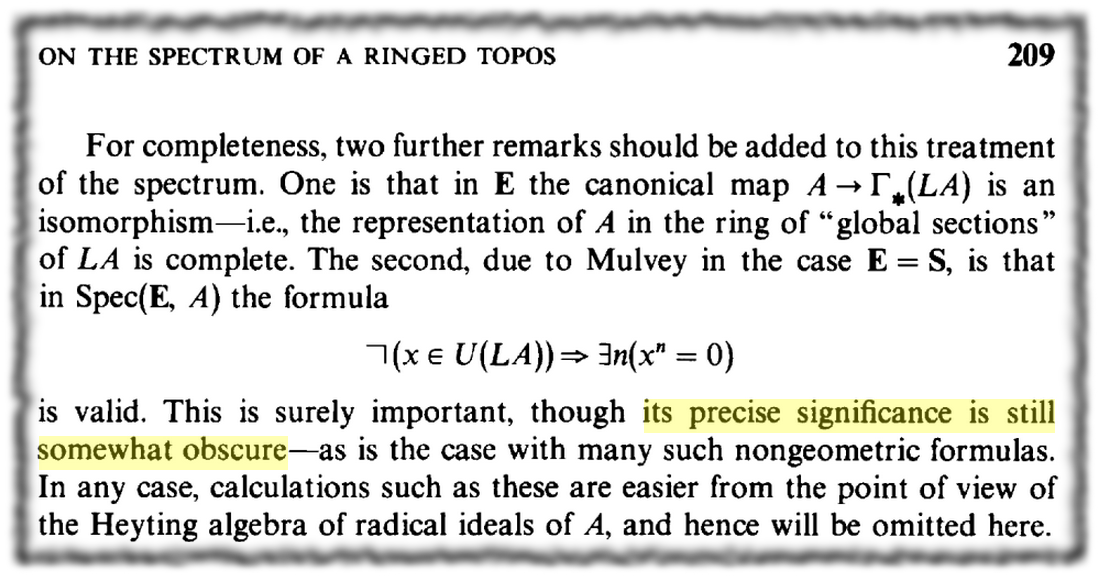
\includegraphics[width=0.9\textwidth]{tierney-on-the-spectrum-of-a-ringed-topos} \\
        \footnotesize
        Miles Tierney. On the spectrum of a ringed topos. 1976.
      }

      \only<4>{
	\begin{varblock}{\textwidth}{}
	  The external meaning of
	  \[
	    \models
	      \speak{$A^\sim[X_1,\ldots,X_n]$ is anonymously Noetherian}
	  \]
	  is:
	  \medskip

	  \begin{indentblock}
	  For any element~$f \in A$ and any (not necessarily quasicoherent) sheaf of
	  ideals~$\J \hookrightarrow A^\sim[X_1,\ldots,X_n]|_{D(f)}$: If
	  \begin{indentblock}
	  for any element~$g \in A$ the condition that
	  \begin{indentblock}
	  the sheaf~$\J$ is of finite type on~$D(g)$
	  \end{indentblock}
	  implies that~$g = 0$,
	  \end{indentblock}
	  then~$f = 0$.
	  \end{indentblock}
	\end{varblock}

	\vspace*{-2em}
      }
    }};
  \end{tikzpicture}}
\end{frame}
\renewcommand{\insertframeextra}{}


\section{Revisiting the test cases}
\setbeamertemplate{headline}{\mynav{gray}{gray}{black}}

\begin{frame}{Revisiting the test cases}
  \vspace*{-1em}
  Let~$A$ be a reduced commutative ring ($x^n = 0 \Rightarrow x = 0$). \\
  Let~$A^\sim$ be its mirror image in the little Zariski topos.

  \begin{columns}[t]
    \begin{column}[t]{0.48\textwidth}
      \centering

      \scalebox{0.5}{$\begin{pmatrix}
        \cdot & \cdot & \cdot & \cdot & \cdot \\
        \cdot & \cdot & \cdot & \cdot & \cdot \\
        \cdot & \cdot & \cdot & \cdot & \cdot
      \end{pmatrix}$}
      \vspace*{-0.5em}

      \begin{varblock}{\textwidth}{A baby example}
        \justifying
        Let~$M$ be an injective matrix over~$A$ with more columns than rows.
        Then~$1 = 0$ in~$A$.
      \end{varblock}

      \justifying
      \textbf{Proof.} $M$ is also injective as a matrix over~$A^\sim$.
      Since~$A^\sim$ is a field, this is a contradiction by basic linear
      algebra. Thus~$\models \bot$. This amounts to~$1 = 0$ in~$A$.
    \end{column}

    \begin{column}[t]{0.57\textwidth}
      \centering

      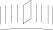
\includegraphics[height=1.9em]{generic-freeness}
      \vspace*{-0.5em}

      \begin{varblock}{\textwidth}{Generic freeness\phantom{p}}
        \justifying
        Let~$M$ be a finitely generated~$A$-module.
        If~$f = 0$ is the only element of~$A$ such that~$M[f^{-1}]$ is a
        free~$A[f^{-1}]$-module, then~$1 = 0$ in~$A$.
      \end{varblock}
      \vspace*{-0.1em}

      \justifying
      \textbf{Proof.} The claim amounts to \mbox{$\models
      \text{``$M^\sim$}$}$\text{
      is \hil{not not} free''}$. Since~$A^\sim$ is a field, this follows from
      basic linear algebra.
    \end{column}
  \end{columns}

  \jnote{1}{With the baby example, we see that the new reduction technique
  presented in this talk allows to reinterpret the core content of the
  classical proof shown on slide~1 in a constructive fashion. Since the forcing
  model was set up in a constructive way, we could mechanically extract an
  explicit procedure from the new proof.

  For the second example, a remark might be in order. A basic theorem of
  undergraduate linear algebra is that any finitely generated vector space has
  a basis. In this form, the theorem cannot quite be proven intuitionistically.
  Indeed, the standard proof uses the law of excluded middle in the first step:
  \begin{indentblock}
    \scriptsize
    Let~$(x_1,\ldots,x_n)$ be a given finite generating family.
    It might be the case that one of the vectors~$x_i$ can be expressed as a
    linear combination of the others, or not.
    In the second case, the family is linearly independent and thus the vector
    space is shown to have a basis.
    In the first case, we continue with the smaller generating
    family~$(x_1,\ldots,x_{i-1},x_{i+1},\ldots,x_n)$ in an inductive fashion.
  \end{indentblock}
  Intuitionistically, the law of excluded middle is not available; however its
  double negation ($\neg\neg(\varphi \vee \neg\varphi)$) is. Threading the
  double negation through the rest of the proof yields the following theorem of
  intuitionistic linear algebra: Any finitely generated vector space is
  \emph{not not} free. It is this theorem which the proof on the slide refers
  to.}
\end{frame}


\backupstart
\setbeamertemplate{headline}{\mynav{gray}{gray}{gray}}

{\usebackgroundtemplate{\begin{minipage}{\paperwidth}\vspace*{4.95cm}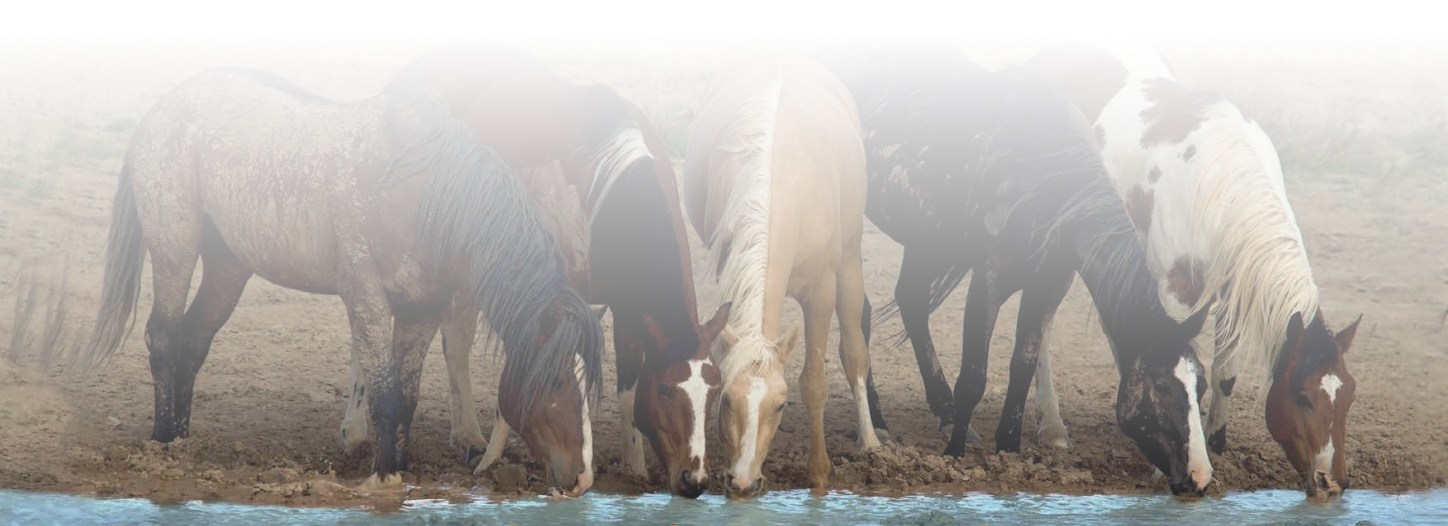
\includegraphics[width=\paperwidth]{topos-horses}\end{minipage}}
\begin{frame}
  \bigskip
  \centering
  
\includegraphics[height=3em]{heart}
  \par
  \raggedright

  The Zariski topos and related toposes have applications in:
  \begin{itemize}
    \item classical algebra and classical algebraic geometry
    \item constructive algebra and constructive algebraic geometry
    \item synthetic algebraic geometry (``schemes are just sets'')
  \end{itemize}

  Connections with:
  \begin{itemize}
    \item understanding quasicoherence
    \item the age-old mystery of nongeometric sequents
  \end{itemize}

  \jnote{1}{Summarizing, we can associate to any reduced ring~$A$ the forcing
  model~$A^\sim$.
  \begin{itemize}
    \item The forcing model has the pleasant property that it is a field.
    \item Reasoning about it requires that we restrict ourselves to
    intuitionistic logic.
  \end{itemize}
  Depending on the application, this trade-off can not be useful at all, or be
  quite valuable. It certainly is so for proving Grothendieck's generic
  freeness lemma, simplifying a multi-page argument to a single and conceptual
  paragraph. (The previous slide only showed a fragment of the general
  statement of Grothendieck's generic freeness lemma. The technique outlined in
  these slides is amenable to the full version. Details are in Section~11.5 of
  \fixedhref{https://rawgit.com/iblech/internal-methods/master/notes.pdf}{these
  notes}.)

  The ideas underlying this new reduction technique can also be used for
  different purposes: for understanding, in a rigorous way, notions of algebraic
  geometry as notions of algebra, and for developing a synthetic account of
  algebraic geometry. This is very briefly touched upon on the next two
  slides.}

  \jnote{2}{
    \centering
    \hil{Further reading}
    \medskip

    \framebox{\fixedhref{https://pizzaseminar.speicherleck.de/skript2/zariski-topos-klein.pdf}{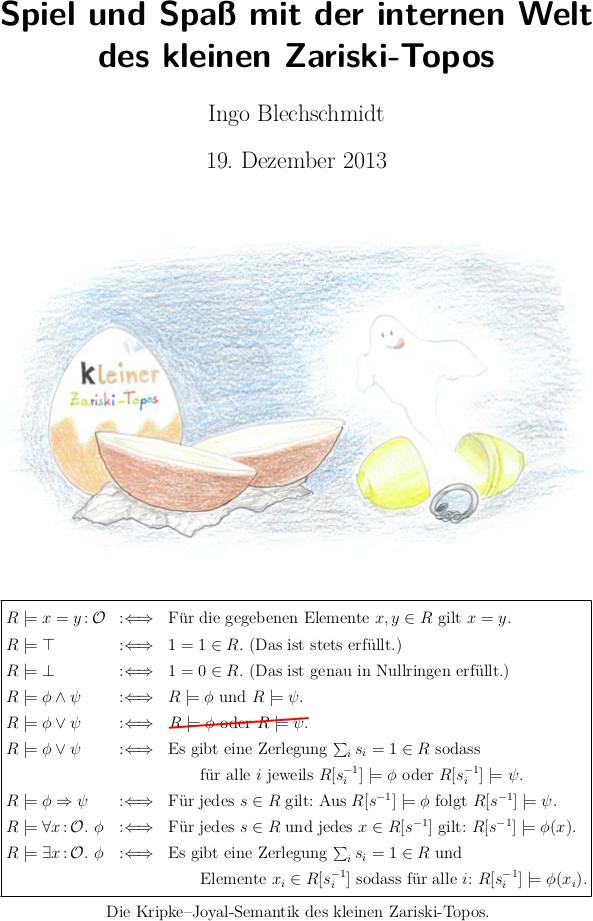
\includegraphics[height=0.8\textheight]{fun-with-the-zariski-topos}}}\qquad%
    \framebox{\fixedhref{https://rawgit.com/iblech/internal-methods/master/notes.pdf}{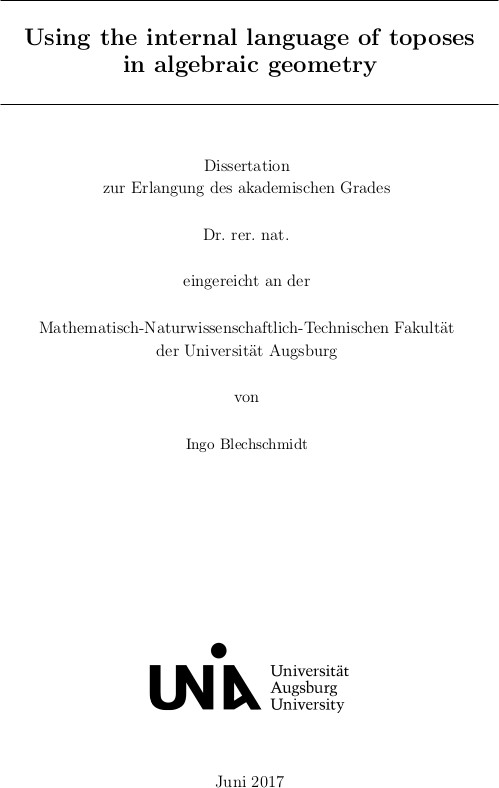
\includegraphics[height=0.8\textheight]{phd-cover}}}
    \par
  }
\end{frame}}

\begin{frame}{Applications in algebraic geometry}
  \vspace*{-1.5em}
  \begin{varblock}{0.9\textwidth}{}
    \justifying
    Understand \hil{notions of algebraic geometry} over a scheme~$X$ as
    \hil{notions of algebra} internal to~$\Sh(X)$.
  \end{varblock}

  \small\centering
  \scalebox{0.83}{\begin{tabular}{ll}
    \toprule
    externally & internally to $\Sh(X)$ \\
    \midrule
    sheaf of sets & set \\
    %sheaf of rings & ring \\
    sheaf of modules & module \\
    sheaf of finite type & finitely generated module \\
    % finite locally free sheaf & finite free module \\
    % coherent sheaf & coherent module \\
    tensor product of sheaves & tensor product of modules \\
    % sheaf of Kähler differentials & module of Kähler differentials \\
    sheaf of rational functions & total quotient ring of~$\O_X$ \\
    dimension of $X$ & Krull dimension of~$\O_X$ \\
    spectrum of a sheaf of~$\O_X$-algebras & ordinary spectrum [with a twist] \\
    higher direct images & sheaf cohomology \\
    \bottomrule
  \end{tabular}}

  \begin{columns}[c]
    \begin{column}{0.47\textwidth}
      \begin{exampleblock}{}
        \justifying
        Let $0 \to \F' \to \F \to \F'' \to 0$ be a short exact sequence
        of sheaves of~$\O_X$-modules. If~$\F'$ and~$\F''$ are of finite type,
        so is~$\F$.
      \end{exampleblock}
    \end{column}

    \begin{column}{0.1\textwidth}
      \vspace*{0.7em}
      \scalebox{3}{$\Leftarrow$}
    \end{column}

    \begin{column}{0.44\textwidth}
      \begin{exampleblock}{}
        \justifying
        Let~$0 \to M' \to M \to M'' \to 0$ be a short exact sequence of
        modules. If~$M'$ and~$M''$ are finitely generated, so is~$M$.
      \end{exampleblock}
    \end{column}
  \end{columns}

  \jnote{1}{One doesn't need to be an expert in topos theory in order to know
  that many notions in algebraic geometry are inspired by notions in algebra
  and that proofs in algebraic geometry often proceed by reducing to algebra.

  If~$X$ is a scheme, the internal language of the topos~$\Sh(X)$ is a way of
  making this connection precise: In many cases, the former are simply
  interpretations of the latter internal to~$\Sh(X)$. Because this connection
  is precise instead of informal, additional value is gained: We can skip many
  basic proofs in algebraic geometry because they're just externalizations of
  proofs in algebra carried out internally to~$\Sh(X)$.}

  \jnote{2}{A basic example is as follows. A short exact sequence of sheaves of
  modules looks like a short exact sequence of plain modules from the internal
  point of view of~$\Sh(X)$. If the two outer sheaves are of finite type, then
  from the internal point of view, the two outer modules will look like
  finitely generated modules. Because the standard proof of the proposition
  quoted on the lower right is intuitionistically valid, it follows that, from
  the internal point of view, the middle module is too finitely generated.
  Consulting the dictionary a second time, this amounts to saying that the
  middle sheaf is of finite type.

  A more advanced example is: The theorem ``any finitely generated vector space
  does \emph{not not} have a basis'' of constructive linear algebra entails, by
  interpretation in~$\Sh(X)$, that any sheaf of finite type over a reduced
  scheme is finite locally free on a \emph{dense open subset}.

  More details on this research program can be found in
  \fixedhref{https://rawgit.com/iblech/internal-methods/master/notes.pdf}{these
  notes}, partly reported on at the
  \fixedhref{https://www.youtube.com/watch?v=7S8--bIKaWQ}{2015 IHÉS topos
  theory conference}. Even though many important dictionary entries are still
  missing (for instance pertaining to derived categories and intersection
  theory), I believe that it is already in its current form useful to working
  algebraic geometers.

  The next slide illustrates a further, different way of approaching algebraic
  geometry using topos theory.}
\end{frame}

\begin{frame}{Synthetic algebraic geometry}
  Usual approach to algebraic geometry: \hil{layer schemes above ordinary set theory}
  using either
  \begin{itemize}
    \item locally ringed spaces
    \small
    \begin{multline*}
      \text{set of prime ideals of~$\ZZ[X,Y,Z]/(X^n+Y^n-Z^n)$} + {} \\
      \text{Zariski topology} + \text{structure sheaf}
    \end{multline*}
    \normalsize
    \item or Grothendieck's functor-of-points account, where a scheme is a functor~$\mathrm{Ring} \to \mathrm{Set}$.
    \small\[ A \longmapsto \{ (x,y,z) \in A^3 \,|\, x^n+y^n-z^n=0 \} \]
  \end{itemize}
  \bigskip

  \jnote{1}{At the
  \fixedhref{https://sbseminar.wordpress.com/2009/08/06/algebraic-geometry-without-prime-ideals/}{Secret
  Blogging Seminar}, there was an insightful long-running discussion on the
  merits of the two approaches to algebraic geometry. Two disadvantages of the approach using
  locally ringed spaces is that the underlying topological spaces don't
  actually parametrize ``honest'', ``geometric'' points, but the more complex
  notion of irreducible closed subsets; and that they don't work well in a
  constructive setting. (For this, they would have to be replaced by locally
  ringed locales.)

  The functorial approach is more economical, philosophically rewarding, and
  works constructively. Given a functor~$F : \Ring \to \Set$, we imagine~$F(A)$
  to be the set of~``$A$-valued points'' of the hypothetical scheme described
  by~$F$, the set of ``points with coordinates in~$A$''. These sets have direct
  geometric meaning. However, typically only field-valued points are easy
  to describe. For instance, the functor representing projective~$n$-space is
  given on fields by
  \[ \begin{array}{r@{}c@{}l}
  K &{}\longmapsto{}& \text{the set of lines through the origin in~$K^{n+1}$} \\
  && \qquad \cong \{ [x_0 \hg \cdots \hg x_n] \,|\, \text{$x_i \neq 0$ for some~$i$} \},
  \end{array} \]
  whereas on general rings it is given by
  \[ \begin{array}{r@{}c@{}l}
    A &{}\longmapsto{}& \text{the set of quotients~$A^{n+1} \twoheadrightarrow P$,
    where~$P$ is projective,} \\
    && \qquad \text{modulo isomorphism}.
  \end{array} \]
  It is these more general kinds of points which impart a sense of
  cohesion on the field-valued points, so they can't simply be dropped from
  consideration.\bigskip}

  \pause

  \hil{Synthetic approach:} model schemes \hil{directly as sets} in a certain
  nonclassical set theory, the internal universe of the \mbox{\hil{big Zariski
  topos}} of a base scheme.
  \small
  \[ \{ (x,y,z) \? (\affl)^3 \,|\, x^n+y^n-z^n=0 \} \]

  \jnote{2}{This tension is resolved by observing that the category of
  functors~$\Ring \to \Set$ is a topos (the \emph{big Zariski topos} of~$\Spec(\ZZ)$)
  and that we can therefore employ its internal language. This language takes
  care of juggling stages behind the scenes. For instance, projective~$n$-space
  can be described by the naive expression
  \[ \{ (x_0,\ldots,x_n) : (\affl)^{n+1} \,|\, x_0 \neq 0 \vee \cdots \vee x_n
  \neq 0 \}/(\affl)^\times. \]
  This example illustrates the goal: to develop a synthetic account of
  algebraic geometry, in which schemes are plain sets and morphisms between
  schemes are maps between those sets. It turns out that there are many
  similarities with the well-developed synthetic account of differential
  geometry, but also important differences, and it also turns out that
  synthetic algebraic geometry has close connections to a certain age-old
  unsolved problem in topos theory, the \emph{mystery of nongeometric
  sequents}.

  Details are in
  \fixedhref{https://rawgit.com/iblech/internal-methods/master/slides-como2018.pdf}{this
  set of slides}.}
\end{frame}

\backupend

\end{document}
